\documentclass[xcolor=pdftex,x11names,table,hyperref]{beamer}

\usepackage{verbatim}
\usepackage{setspace}
\usepackage{graphbox}
\usepackage{url}
\usepackage{xcolor} % See documentation PDF at http://www.ctan.org/pkg/xcolor
\definecolor{darkgreen}{rgb}{0,0.3,0}
\definecolor{darkblue}{rgb}{.05,.05,.30}
\definecolor{lightgrey}{rgb}{0.65,0.65,0.65}
\usepackage{tikzsymbols}


\setbeamertemplate{section in toc}[sections numbered]
\setbeamertemplate{subsection in toc}[subsections numbered]
\setbeamertemplate{subsubsection in toc}[subsubsections numbered]
\usetheme{Singapore}
\setbeamertemplate{navigation symbols}{}
\setbeamertemplate{footline}{%
\vspace{0.0em}%
\hspace{0.5em}%
{\color[rgb]{.1,.1,.1} \insertframenumber{}~/~\inserttotalframenumber}
}

\newcommand{\code}[1]{{\color{darkgreen}\texttt{#1}}}
\newcommand{\detail}[1]{{\color{lightgrey}\small{}#1}}
\newcommand{\teeny}[1]{\scalebox{0.17}{#1}}
\newcommand{\tablecolors}{\rowcolors{2}{blue!12}{white}} % Cool table colors

\newcommand{\actfun}[1]{\includegraphics[height=0.11\textheight,align=c]{images/#1}} % For consistency

\begin{document}

\title{Neural Nets \\[1.5em]
 %
\includegraphics[width=0.5\textwidth]{images/kitten_string_flickr_albaraa.jpg} \\[-1.0em]
 \small{Part 1} \\[1.0em]
 %LT1 \\[1.0em]
 }
\author{\href{http://jon.dehdari.org}{Jon Dehdari}}
\frame{\titlepage}

\begin{frame}{Good Morning!}
	\begin{center}
	%\includegraphics[width=0.8\textwidth]{images/.jpg}
	\end{center}
\end{frame}

% extension of maxent models
\begin{frame}{Logistic Regression (=Softmax Regression)}
\begin{itemize}
	\item {\small Recall that \textbf{logistic regression} involves the dot product of an input vector and a weight matrix, then a normalized sigmoid function (softmax)}
	\pause
	\item A \textbf{feedforward neural network} just adds one or more layers between the input vector and the softmax output
	\pause
	\begin{center}
	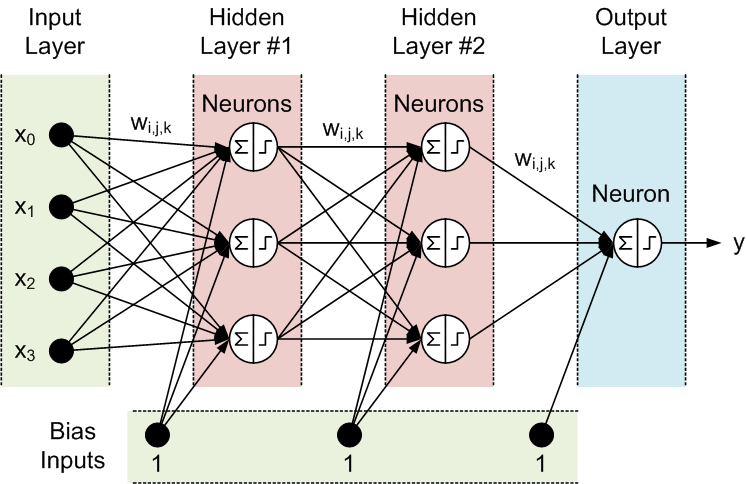
\includegraphics[height=0.58\textheight]{images/nnet_mql5.png}
	\end{center}
\end{itemize}
\teeny{Courtesy of \href{https://www.mql5.com/en/code/9002}{mql5.com}}
\end{frame}

% what can they do that maxent can't: 
% Universal approximation theorem (George Cybenko, 1989) non-linear representations.  One hidden layer: any continuous function. Two hidden layers: any discontinuous function
% https://www.mql5.com/en/code/9002
\begin{frame}{Why Use Hidden Layers?}
\begin{itemize}
	\item In contrast to log-linear models, neural networks can have \textbf{non-linear} representations of data
	\item The \textbf{\href{https://en.wikipedia.org/wiki/Universal_approximation_theorem}{universal approximation theorem}} (George Cybenko, 1989) found that a neural network with one hidden layer can approximate \textbf{any continous function}
	\item A network with two hidden layers can represent discontinuous functions
	\begin{center}
	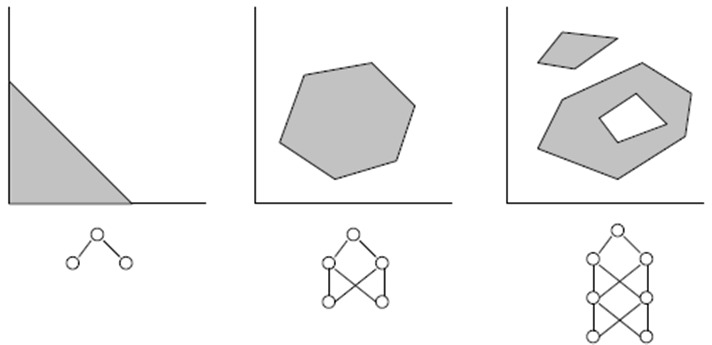
\includegraphics[height=0.42\textheight]{images/nnet_mql5_function_approximations.png}
	\end{center}
\end{itemize}
\teeny{Courtesy of \href{https://www.mql5.com/en/code/9002}{mql5.com}}
\end{frame}

% activation functions: linear, relu, heaviside step function, tanh, logistic, softmax
\begin{frame}{Activation Functions}
	In each layer, the output of the dot product goes through an \textbf{\href{https://en.wikipedia.org/wiki/Activation_function}{activation function}}. Here are some examples: \\[0.3em]
\begin{footnotesize}
\begin{spacing}{0.85}
\hspace*{-3.0em}%
\begin{tabular}{lllp{0.38\textwidth}}
	\bf Name & \bf Visualization & $\bf f(x)=$ & \bf Notes \\
	\hline
	Linear  (= Identity) & \actfun{activation_linear_wp.png} & $x$ & Not useful for hidden layers \\
	Heaviside Step & \actfun{activation_heaviside_step_wp.png} & {\tiny $ \left \{\begin{array}{rcl} 0 & \mbox{for} & x < 0\\ 1 & \mbox{for} & x \ge 0\end{array} \right. $ }  \hspace*{-1.0em} & Not differentiable \\
{\scriptsize Rectified Linear (ReLU)} & \actfun{activation_relu_wp.png} & {\tiny $ \left \{\begin{array}{rcl} 0 & \mbox{for} & x < 0 \\ x & \mbox{for} & x \ge 0\end{array} \right.$ } \hspace*{-1.0em} & Surprisingly useful in practice \\
	Tanh & \actfun{activation_tanh_wp.png} & $\frac{2}{1+e^{-2x}}-1$ & A soft step function; ranges from -1 to 1 \\
	Logistic & \actfun{activation_logistic_wp.png} & $\frac{1}{1+e^{-x}}$ & Another soft step function; ranges from 0 to 1 \\
	Softmax & \actfun{activation_logistic_wp.png} & $\frac{e^{\boldsymbol W_y \cdot \mathbf{x}} }{Z} $ & Normalized sigmoidal function. Useful for last layer when training on cross entropy \\
\end{tabular}
\end{spacing}
\end{footnotesize}
\end{frame}

% training them via backprop: why, how;
\begin{frame}{}
\begin{itemize}
	\item 
	\item 
\end{itemize}
\end{frame}

% autoencoders, classifiers
\begin{frame}{}
\begin{itemize}
	\item 
	\item 
\end{itemize}
\end{frame}

% loss functions
\begin{frame}{}
\begin{itemize}
	\item 
	\item 
\end{itemize}
\end{frame}

% discussion of depth, width, dropout, early stopping based on dev set
\begin{frame}{}
\begin{itemize}
	\item 
	\item 
\end{itemize}
\end{frame}

% discussion of softmax, class-based decomp, hier softmax
\begin{frame}{}
\begin{itemize}
	\item 
	\item 
\end{itemize}
\end{frame}

% software: theano-based, tensorflow-based, torch-based, others (Caffe, CNN, ...)
\begin{frame}{}
\begin{itemize}
	\item 
	\item 
\end{itemize}
\end{frame}

% automatic differentiation of graph, why it's nice
\begin{frame}{}
\begin{itemize}
	\item 
	\item 
\end{itemize}
\end{frame}

% Second set: recurrent NN's (Elman, GRU, LSTM), BPTT, maybe convolutional nets

\begin{frame}{}
\begin{itemize}
	\item 
	\item 
\end{itemize}
\end{frame}





% \begin{frame}{}
% \begin{itemize}
% 	\item 
% 	\item 
% 	\item 
% \end{itemize}
% \end{frame}


\end{document}
